\chapter{Vorgehen}

\section{Inbetriebnahme Prototyp}

\subsubsection{Senden Geschwindigkeit per BLE}
Funktioniert bei einer Geschwindigkeit von 70 km/h. 

\begin{figure}[h!]
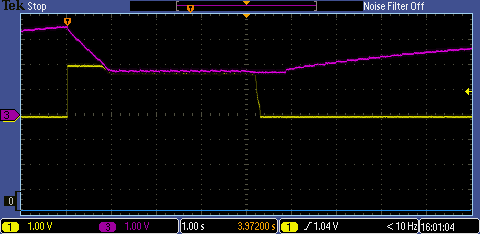
\includegraphics[bb=0 240 50 50]{EnergieSenden.PNG}
\caption{Prototyp Ausgangsspannung Energy Management Board}
\end{figure}

\newpage 

Nachmessen der Energie Spule:

Es braucht hohe Geschwindigkeit.

Neue Spule gestestet.


\begin{figure}[h]
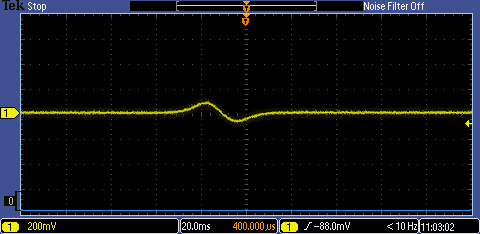
\includegraphics[bb=0 100 50 50]{PremoSpule.PNG}
\caption{Energiegewinnung Premospule}
\end{figure}

\begin{figure}[h]
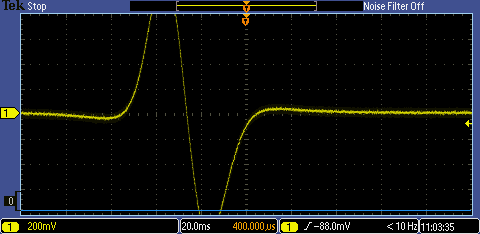
\includegraphics[bb=0 150 50 50]{UnbekannteSpule.PNG}
\caption{Energiegewinnung Unbekannte Spule}
\end{figure}

\pagebreak 
\subsubsection{Messungen Energy Management Board}
Die Applikationsspannung braucht alle Energie. LTS lädt nicht. 
\\

Lastverhalten wie Sensortag

\begin{figure}[h]
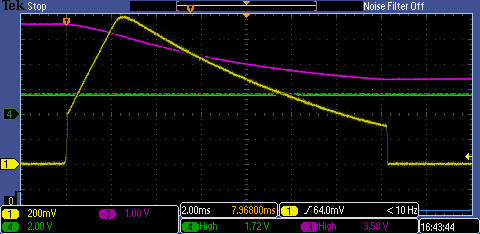
\includegraphics[bb=0 100 50 50]{EMBoardAusgang10Ohm.PNG}
\caption{Ausgangsspannung 10 Ohm}
\end{figure}

\begin{figure}[h]
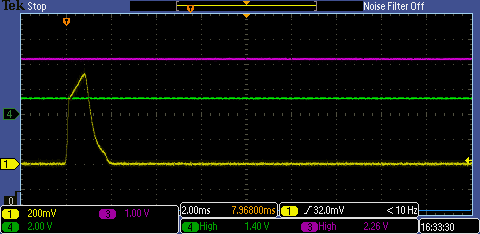
\includegraphics[bb=0 150 50 50]{EMBoardAusgang100Ohm.PNG}
\caption{Energiegewinnung Unbekannte Spule}
\end{figure}



\pagebreak
\subsubsection{Messungen Sensortag}
Ziel: Energieverbrauch kennen.

Unterschied zwischen dem Programmierten Sensortag des Prototypen und dem neuen Sensortag.

\begin{figure}[h]
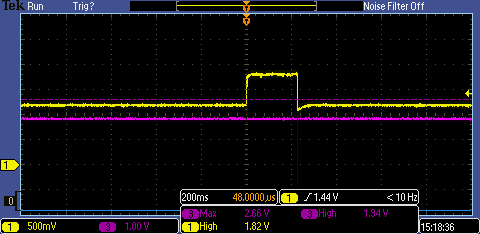
\includegraphics[bb=0 300 50 50]{SensortagRuhestrom.PNG}
\caption{Energieverbrauch (strom) neues Sensortag}
\end{figure}

\begin{figure}[h]
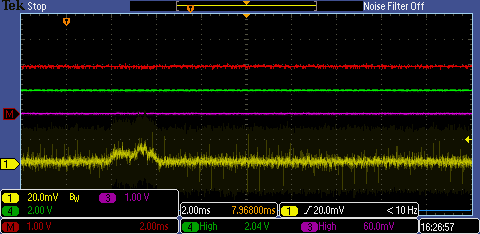
\includegraphics[bb=0 550 50 50]{NeuesSensortagSTromverbrauch.PNG}
\caption{Energieverbrauch Protoyp}
\end{figure}

\textbf{Sensortag Prototyp: defekt ? Auf neues Sensortag Konfiguration neu laden.
}


\section{Layout Print}

\section{Kommunikation Bluetooth Low Energy}

\section{Energieoptimierung}



\section{Applikationsentwicklung}

\section{Option 1}






